\documentclass[xcolor=table, 10pt, aspectratio=169]{beamer}

%\usepackage{arev}
\usepackage{amsmath,amssymb,amscd}
\usepackage{dsfont}
\usepackage{mathrsfs}
\usepackage{yfonts}
\usepackage{bm}
\usepackage{graphicx}
\usepackage{tabularx}
\usepackage{animate}
\usepackage{mathtools}
%\usepackage{ifthen}

%\usepackage{xeCJK}
%\usepackage{fontspec}
%\newfontfamily\cjkfont{PingFang SC}
%\setCJKmainfont{PingFang SC}
\newcolumntype{x}{>{\centering\arraybackslash}X}
\renewcommand{\arraystretch}{1.5}

\usepackage{tikz}
	\usetikzlibrary{calc}
	\usetikzlibrary{arrows,shapes, positioning, matrix}
	\usetikzlibrary{decorations.markings}
	\tikzstyle arrowstyle=[scale=1]
	\tikzstyle directed=[postaction={decorate,decoration={markings,
 	   mark=at position .15 with {\arrow[arrowstyle]{stealth}}}}]
\tikzstyle string=[thick,postaction={decorate,decoration={markings,
    mark=at position .55 with {\arrow[arrowstyle]{stealth}}}}]
\tikzstyle dual_string=[dashed,postaction={decorate,decoration={markings,
    mark=at position .55 with {\arrow[arrowstyle]{stealth}}}}]

\tikzstyle dw=[thick,postaction={decorate,decoration={markings,
    mark=at position 1 with {\arrow[arrowstyle]{stealth}}}}]
\tikzstyle group=[mbg]

\usepackage{pgffor}
\newcommand{\mb}[1]{\mathbf{#1}}
\renewcommand{\cal}[1]{\mathcal{#1}}

\newcommand{\ag}[2]{#1_\mb{#2}}
\newcommand{\cohosub}[1]{\scalebox{0.72}{\textswab{#1}}}
\newcommand{\cohosubsub}[1]{\scalebox{0.6}{\textswab{#1}}}
\newcommand{\coho}[1]{\textswab{#1}}


\mode<presentation>
{
  %\usetheme{Warsaw}
  % or ...
  %\useoutertheme{rectangle}
  \setbeamertemplate{frametitle}[default][center]
  \defbeamertemplate{itemize item}{flat}{\begin{pgfpicture}{-1ex}{0ex}{1ex}{2ex}
      \pgfpathcircle{\pgfpoint{0pt}{.6ex}}{0.6ex}
      \pgfusepath{fill}
    \end{pgfpicture}%
  }
  \defbeamertemplate{itemize subitem}{flat}{\footnotesize\raise0.5pt\hbox{\textbullet}}
  \defbeamertemplate{itemize subsubitem}{flat}{\footnotesize\raise0.5pt\hbox{\textbullet}}

  %\useinnertheme{circles}
  \setbeamertemplate{items}[flat]
  \setbeamertemplate{sections/subsections in toc}[circle]
  \setbeamertemplate{blocks}[rounded]
  \setbeamertemplate{title page}[default][colsep=-4bp,rounded=true]
  \setbeamertemplate{part page}[default][colsep=-4bp,rounded=true]
  \setbeamercovered{transparent}
  %\usecolortheme{spruce}
  %\definecolor{THU}{RGB}{116,61,130}
  \definecolor{mbg}{RGB}{0,0,160}
  \setbeamercolor*{palette primary}{fg=white,bg=mbg}
  \setbeamercolor*{titlelike}{parent=palette primary}
  \setbeamercolor*{structure}{fg=mbg}
  \setbeamercolor{frametitle}{fg=white,bg=mbg}
  % or whatever (possibly just delete it)
  \setbeamercolor{block title}{bg=mbg,fg=white}
  \setbeamercolor{block body}{bg=mbg!15}


  \addtobeamertemplate{navigation symbols}{}{ \hspace{1em}%
    \usebeamerfont{footline}%
    \insertframenumber / \inserttotalframenumber }
}


%\usepackage[english]{babel}
% or whatever

%\usepackage[latin1]{inputenc}
% or whatever

%\usepackage{times}
%\usepackage[T1]{fontenc}
% Or whatever. Note that the encoding and the font should match. If T1
% does not look nice, try deleting the line with the fontenc.

\title[SMLC] % (optional, use only with long paper titles)
{Guiding Monte Carlo Simulations with Machine Learning}

\author[Y Qi] % (optional, use only with lots of authors)
{Yang~Qi}
% - Give the names in the same order as the appear in the paper.
% - Use the \inst{?} command only if the authors have different
%   affiliation.

\institute[Fudan] % (optional, but mostly needed)
{
  Department of Physics, Fudan University
}
% - Use the \inst command only if there are several affiliations.
% - Keep it simple, no one is interested in your street address.

%\date{2016 Annual Meeting of Fudan CFTPP} % (optional, should be abbreviation of conference name)
%{Fudan University, Oct 13 2015}
\date{APS March Meeting 2018.}
% - Either use conference name or its abbreviation.
% - Not really informative to the audience, more for people (including
%   yourself) who are reading the slides online

\subject{Theoretical Physics}
% This is only inserted into the PDF information catalog. Can be left
% out.



% If you have a file called "university-logo-filename.xxx", where xxx
% is a graphic format that can be processed by latex or pdflatex,
% resp., then you can add a logo as follows:

%\pgfdeclareimage[height=1cm]{university-logo}{fudan}
%\logo{\pgfuseimage{university-logo}}



% Delete this, if you do not want the table of contents to pop up at
% the beginning of each subsection:
\AtBeginSection[]
{
  \begin{frame}<beamer>{Outline}
			\tableofcontents[currentsection,currentsubsection]
  \end{frame}
}
%\AtBeginSubsection[]
%{
 % \begin{frame}<beamer>{Outline}
  %  \tableofcontents[currentsection,currentsubsection]
  %\end{frame}
%}


\begin{document}

\begin{frame}
  \titlepage
\end{frame}

\begin{frame}{References}
\begin{itemize}
%\item Works led by Liang Fu, Zi-Yang Meng, and Lei Wang.
\item MIT: Jun-Wei Liu, Hui-Tao Shen, Yuki Nagai, Liang Fu.
\item IOP: Xiao-Yan Xu, Zi-Yang Meng.
\item References:
\begin{enumerate}
  \item J Liu, YQ, Z-Y Meng and L Fu, PRB 95, 041101(R) (2017).
  \item J Liu, H Shen, YQ, Z-Y Meng and L Fu, PRB 95, 241104(R) (2017).
  \item X-Y Xu, YQ, J Liu, L Fu and Z-Y Meng, PRB 96, 041119(R) (2017).
  \item Y Nagai, H Shen, YQ and L Fu, PRB 96, 161102(R) (2017).
\end{enumerate}
\begin{center}
	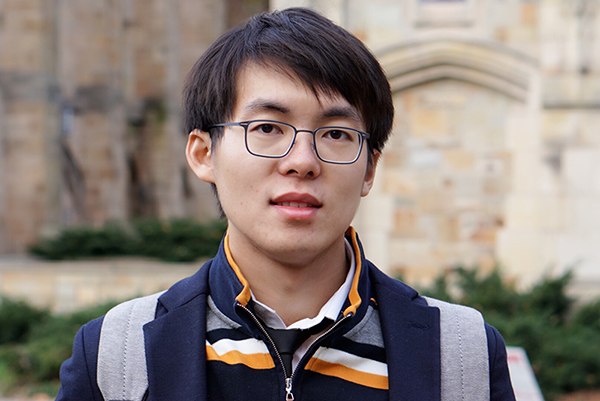
\includegraphics[height=2cm]{../people/huitaoshen}
	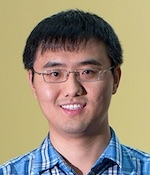
\includegraphics[height=2cm]{../people/junweiliu}
	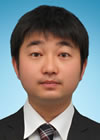
\includegraphics[height=2cm]{../people/yuki}
	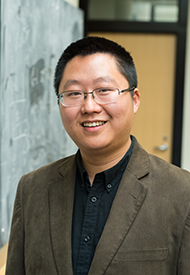
\includegraphics[height=2cm]{../people/liangfu}
	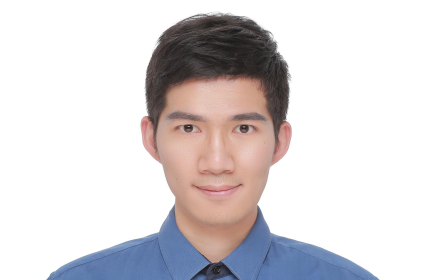
\includegraphics[height=2cm]{../people/xiaoyanxu}
	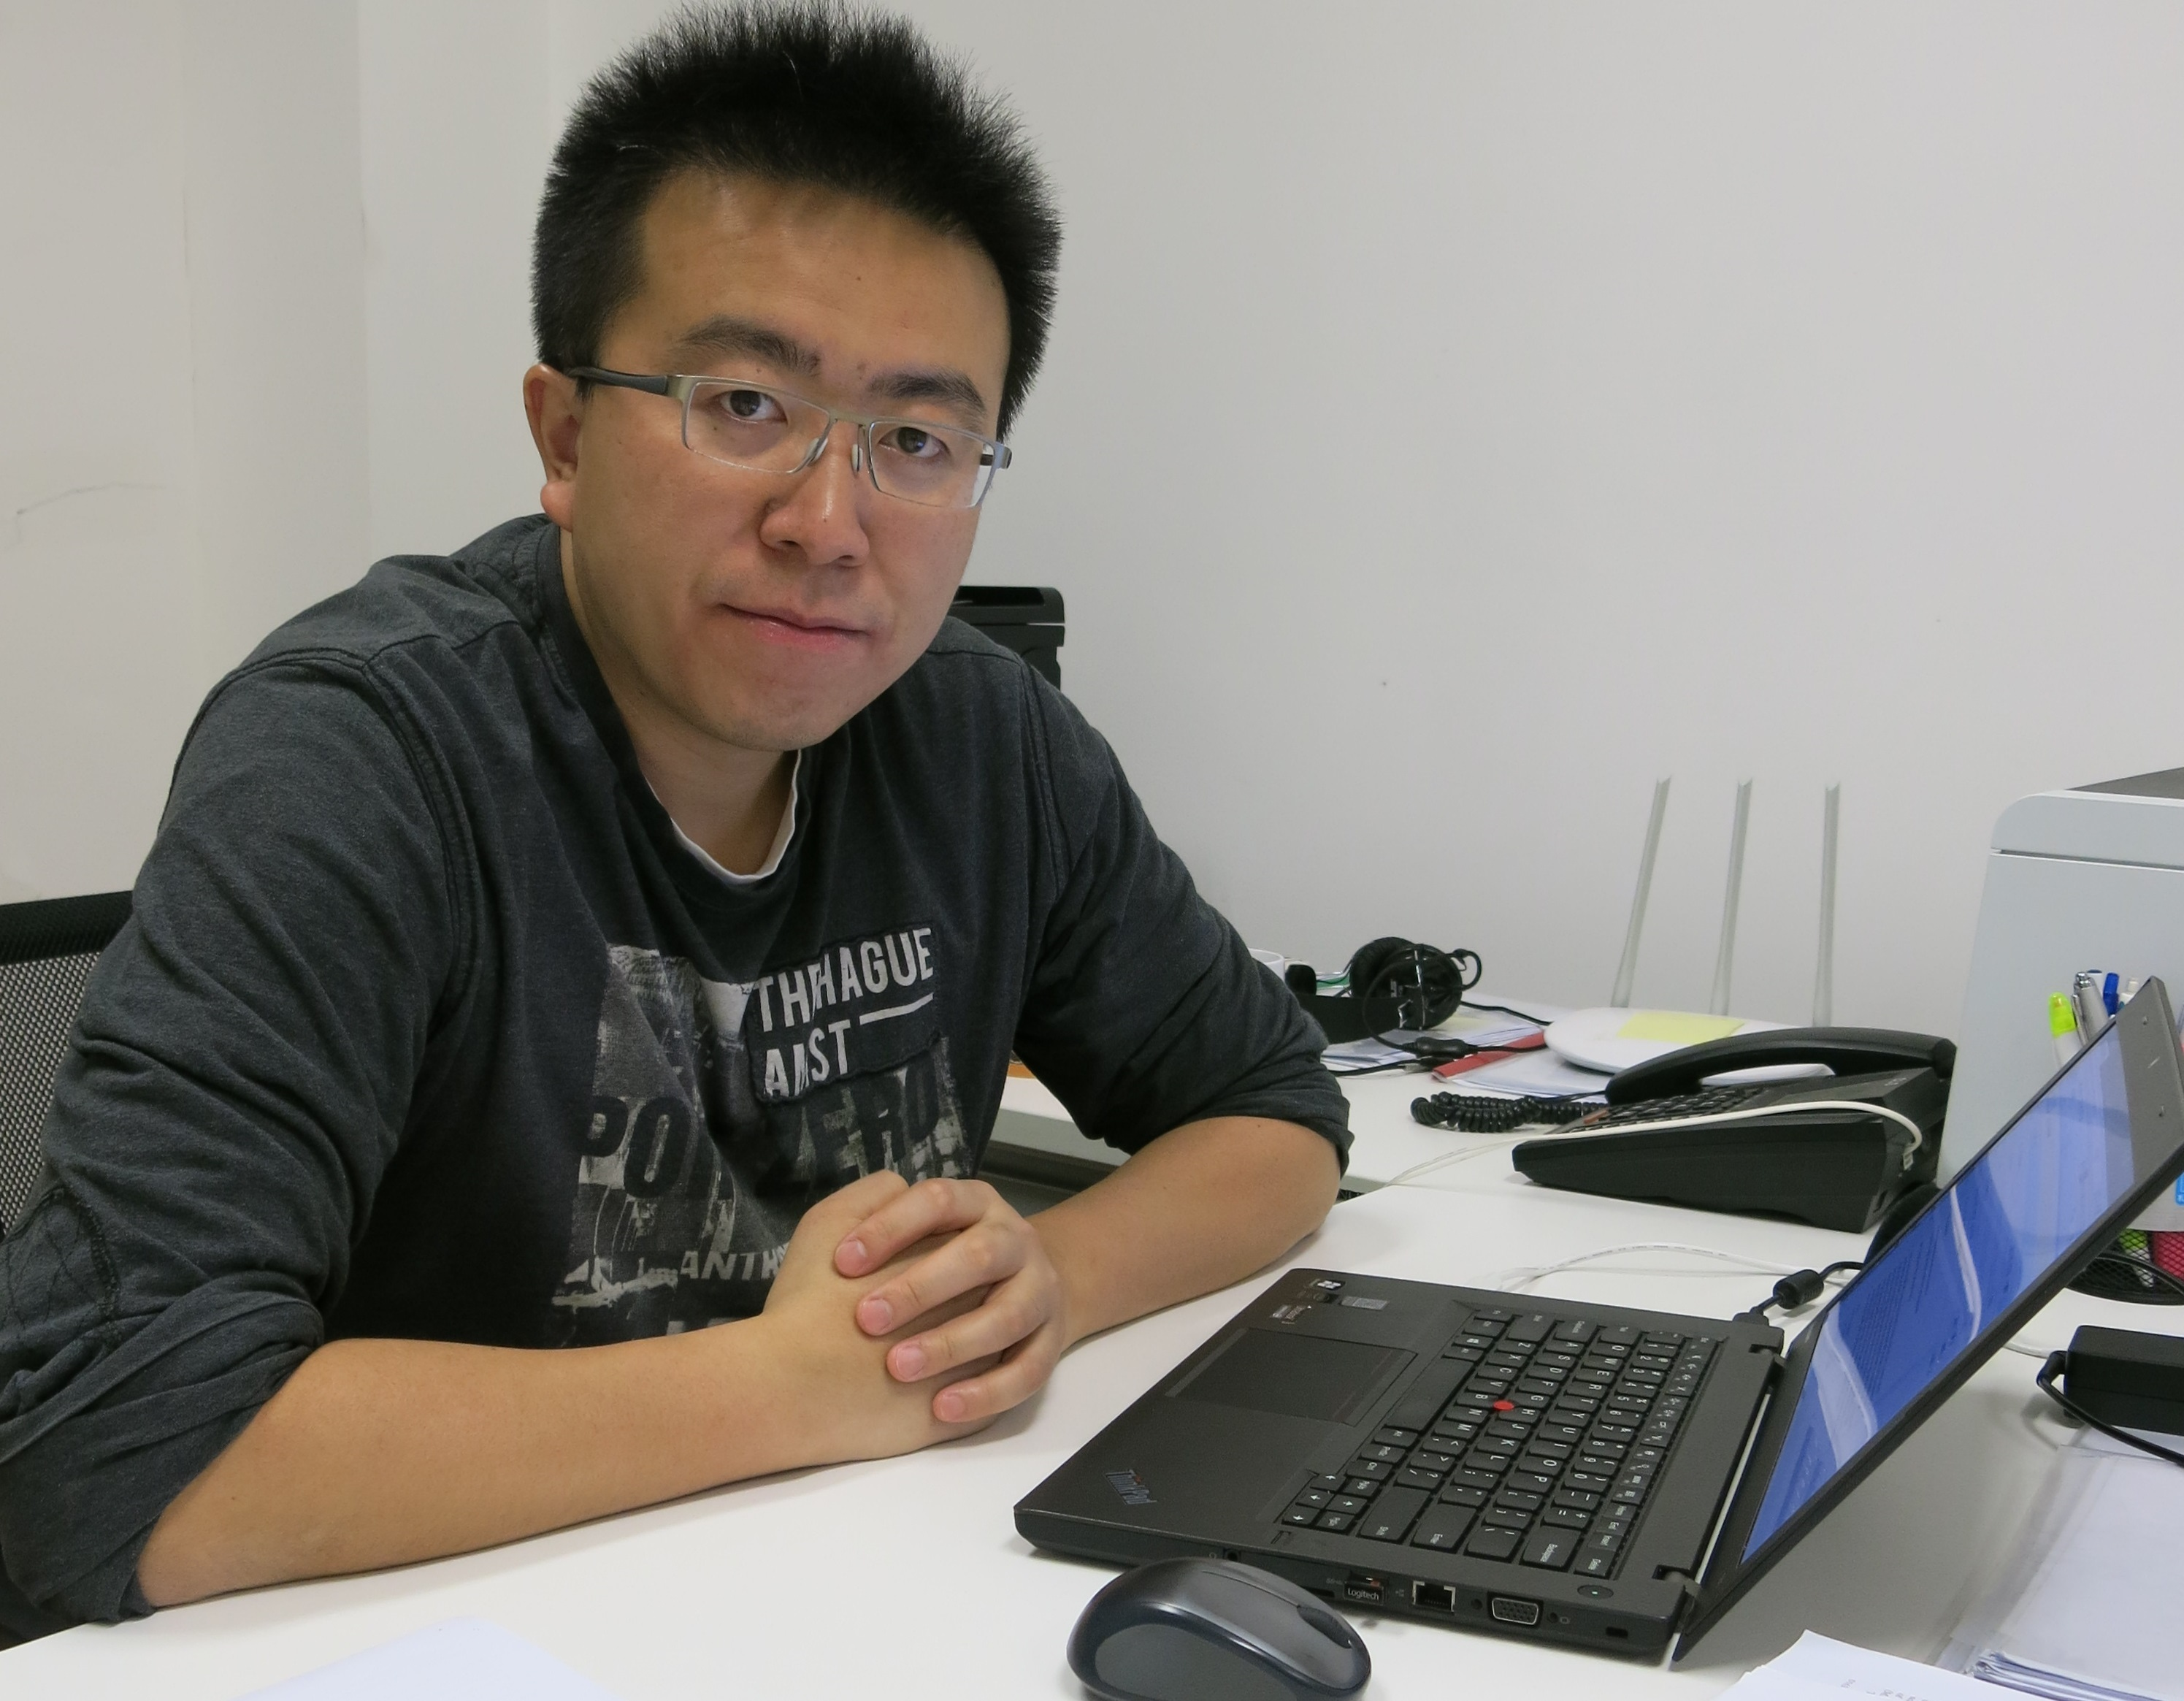
\includegraphics[height=2cm]{../people/ziyangmeng}
\end{center}
\item Related works:
\begin{enumerate}
  \item Li Huang, Lei Wang, PRB 95, 035105(R) (2017).
  \item Li Huang, Yi-Feng Yang, Lei Wang, PRE 95, 031301(R)(2017).
  \item Lei Wang, arXiv:1702.08586 [cond-mat.str-el].
\end{enumerate}
\end{itemize}
\end{frame}

\begin{frame}{Outline}
	%\begin{columns}
	%\column{.7\textwidth}
		\tableofcontents
  %\end{columns}
  % You might wish to add the option [pausesections]
\end{frame}

\section{Introduction to Markov Chain Monte Carlo: the Importance of Update}

\begin{frame}
  \frametitle{Monte Carlo simulation: an unbiased method}
  \begin{itemize}
    \item A widely used numerical method in statistical physics and quantum many-body physics.
    \item Unbiased: reliable statistical error bar.
    \item Fast: error decreases as $1/\sqrt{\mathcal N}$.
    \item Universal: applies to any model without the sign program.
  \end{itemize}
\end{frame}

\begin{frame}
  \frametitle{Introduction to MCMC}
  \begin{itemize}
    \item Consider a statistical mechanics model:
    \[Z=\sum_{\mathcal C}e^{-\beta H[\mathcal C]} = \sum_{\mathcal C}W(\mathcal C).\]
    \item The Markov-chain Monte Carlo (MCMC) is a way to do importance sampling.
    \item A Markov chain is constructed,
    \[\cdots\rightarrow\mathcal C_{i-1}\rightarrow\mathcal C_i\rightarrow\mathcal C_{i+1}\rightarrow\cdots\]
    \item Markov chain: $p(\mathcal C_i\rightarrow\mathcal C_j)$ only depends on $\mathcal C_i$ (no memory).
    \item Goal: distribution of $\mathcal C$ converges to the Boltzmann distribution $W(\mathcal C)$.
    \item Any observable can be measured from a Markov chain,
    \[\langle O\rangle = \frac{\sum O(\mathcal C)W(\mathcal C)}{\sum W(\mathcal C)} \simeq
     \frac1{\mathcal N}\sum_iO(\mathcal C_i).\]
  \end{itemize}
\end{frame}

\begin{frame}
  \frametitle{Detailed balance}
  \begin{itemize}
    \item Detailed balance:
    \[\mathcal C\leftrightarrow\mathcal D,\quad
		\frac{p(\mathcal C\rightarrow\mathcal D)}{p(\mathcal D\rightarrow\mathcal C)}=\frac{W(\mathcal D)}{W(\mathcal C)}.\]
    \item Detailed balance (and ergodicity) guarantees that if the MC converges, it converges to the desired distribution $W(\mathcal C)$.
    \item Metropolis-Hastings algorithm: propose -- accept/reject.
    \[p(\mathcal C\rightarrow\mathcal D) = q(\mathcal C\rightarrow\mathcal D)
    \alpha(\mathcal C\rightarrow\mathcal D).\]
    \[\alpha(\mathcal C\rightarrow\mathcal D) =
    \min\left\{1, \frac{W(\mathcal D)}{W(\mathcal C)}
    \frac{q(\mathcal D\rightarrow\mathcal C)}
    {q(\mathcal C\rightarrow\mathcal D)}\right\}.\]
  \end{itemize}
\end{frame}

\begin{frame}
  \frametitle{Autocorrelation time}
  \begin{itemize}
    \item Autocorrelation time measures the efficiency of the update algorithm.
    \item ``time'' sequence:
    \[\cdots\rightarrow O(t-1)\rightarrow O(t)\rightarrow O(t+1)\rightarrow\cdots,
  \quad O(t) = O[\mathcal C(t)].\]
    \item Autocorrelation function
    \[\mathcal A_O(\Delta t)=\langle O(t)O(t+\Delta t)\rangle - \langle O(t)\rangle^2\propto e^{-\Delta t/\tau}.\]
  \end{itemize}
  \begin{columns}
    \column{.5\textwidth}
    \begin{block}{Complexity $\propto \tau$}
      \[\langle O\rangle = \frac1{\mathcal N}\sum_iO(\mathcal C_i).\]
      Statistical error $\delta O\sim\frac1{\sqrt{\mathcal N}}$ only if $O(i)$ are independent.
    \end{block}
    \column{.5\textwidth}
    \centering
    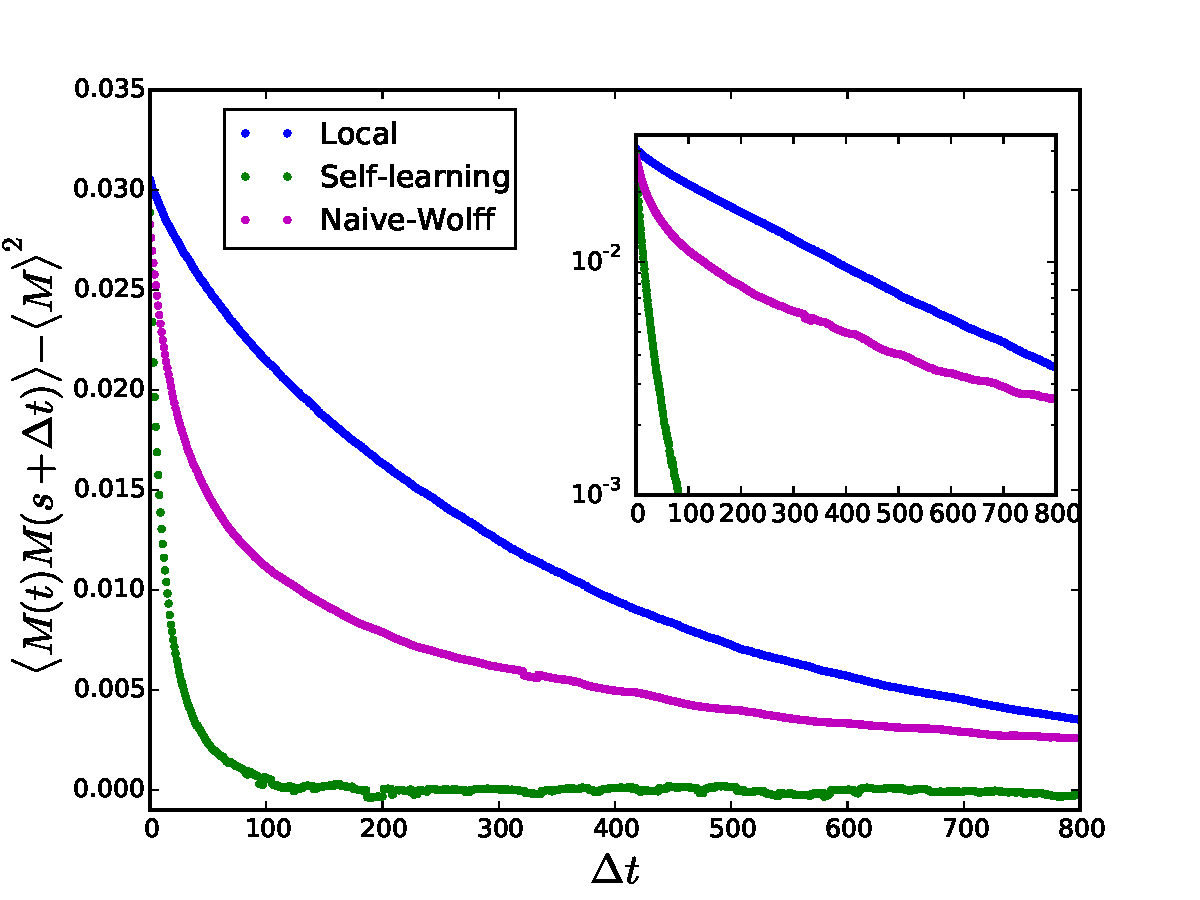
\includegraphics[height=3.5cm]{auto_decay}
  \end{columns}
\end{frame}

\begin{frame}
  \frametitle{Performence of the algorithm}
    \begin{itemize}
      \item Theory
      \begin{center}
        
\includegraphics[height=2.5cm]{laptop_coffee}
      \end{center}
      \item Reality
      \begin{center}
        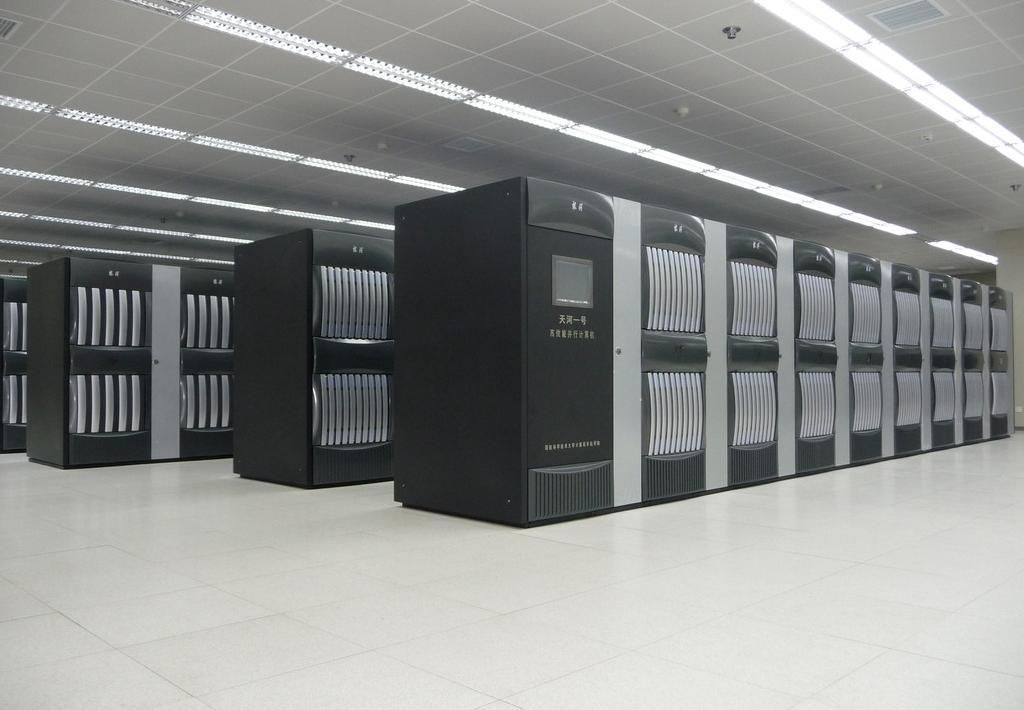
\includegraphics[height=2.5cm]{tianhe}
      \end{center}
      \item Why?
      \[\text{Cost} \propto \text{Cost of each step} \times \text{autocorrelation time}\]
    \end{itemize}
\end{frame}

\begin{frame}
  \frametitle{Local Update: Metropolis algorithm}
  \begin{center}
    \begin{tikzpicture}
      \node<1> at (0, 0) [circle, draw] {};
      \node<2> at (0, 0) [circle, fill, draw] {};
      \node at (1, 0) [circle, draw] {};
      \node at (0, 1) [circle, draw] {};
      \node at (-1, 0) [circle, fill, draw] {};
      \node at (0, -1) [circle, fill, draw] {};
    \end{tikzpicture}
  \end{center}
  \begin{itemize}
    \item Local update: randomly select a site and flip the spin.
    \item $q(\mathcal C\rightarrow\mathcal D) = q(\mathcal D\rightarrow\mathcal C) = \frac1N$.
    \item $\alpha(\mathcal C\rightarrow\mathcal D)=\min\left\{1,\frac{W(\mathcal D)}{W(\mathcal C)}\right\}.$
    \item $N$ trials are counted as one MC step.
    \item Very general: applies to any model.
    \item N Metropolis, A W Rosenbluth, M N Rosenbluth, A H Teller, and E Teller, J Chem Phys \textbf{21}, 1087 (1953).
  \end{itemize}
\end{frame}

\begin{frame}
  \frametitle{Critical slowing down}
  \begin{itemize}
    \item The real dynamical relaxation time diverges at the critical point: a critical system is slow to equilibrate.
    \item The local update mimics the real relaxation process: also exhibits the critical slowing down phenomena.
    \item $\tau\propto L^z$, $z=2.125$ for the 2D Ising model.
  \end{itemize}
  \begin{center}
    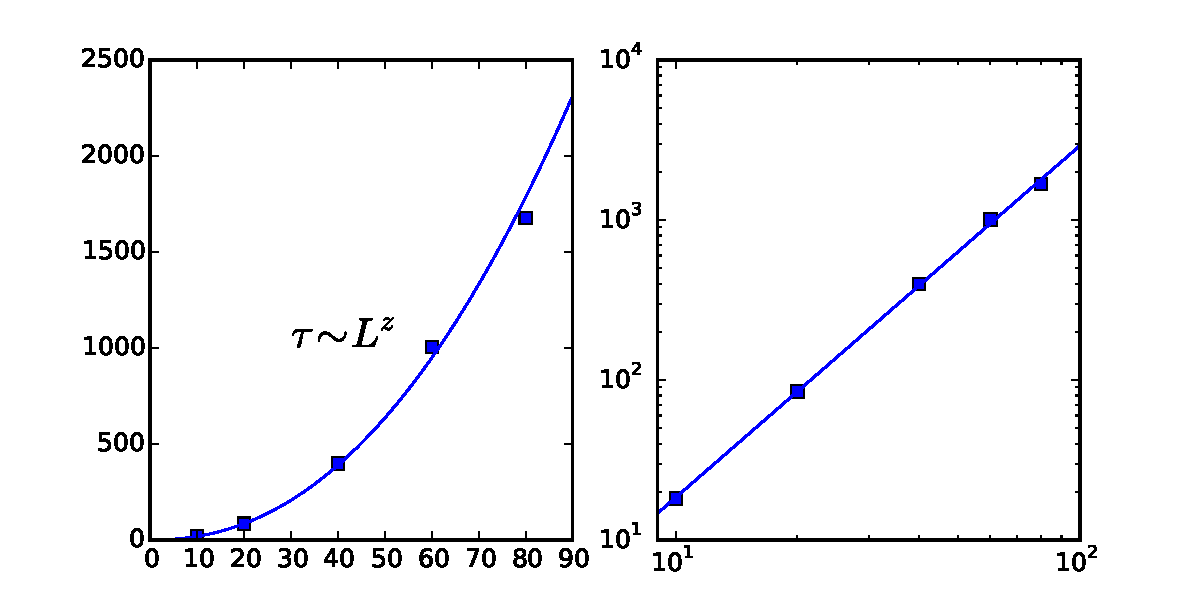
\includegraphics[width=8cm]{slowdown}
  \end{center}
  There's a way around this: MCMC simulation does not have to mimic the real dynamics...
\end{frame}

\begin{frame}
  \frametitle{Wolff algorithm: a cluster update}
  \begin{center}
    \begin{tikzpicture}[scale=.8]
      \node (v00) at (0, 0) [circle, draw] {};
      \node (v10) at (1, 0) [circle, draw] {};
      \node (v20) at (2, 0) [circle, draw] {};
      \node (v30) at (3, 0) [circle, fill, draw] {};

      \node (v01) at (0, 1) [circle, fill, draw] {};
      \node (v11) at (1, 1) [circle, draw] {};
      \node (v21) at (2, 1) [circle, draw] {};
      \node (v31) at (3, 1) [circle, fill, draw] {};

      \node (v02) at (0, 2) [circle, draw] {};
      \node (v12) at (1, 2) [circle, draw] {};
      \node (v22) at (2, 2) [circle, fill, draw] {};
      \node (v32) at (3, 2) [circle, draw] {};

      \node (v03) at (0, 3) [circle, draw] {};
      \node (v13) at (1, 3) [circle, draw] {};
      \node (v23) at (2, 3) [circle, fill, draw] {};
      \node (v33) at (3, 3) [circle, draw] {};

      \node<8> at (1, 1) [circle, fill, draw] {};
      \draw<2> (v11) -- (v12) [dashed];
      \draw<3-> (v11) -- (v12);
      \node<8> at (1, 2) [circle, fill, draw] {};
      \draw<4> (v12) -- (v13) [dashed];
      \draw<5-> (v12) -- (v13);
      \node<8> at (1, 3) [circle, fill, draw] {};
      \draw<6> (v12) -- (v02) [dashed];
      \draw<7-> (v11) -- (v10);
      \node<8> at (1, 0) [circle, fill, draw] {};
      \draw<7-> (v11) -- (v21);
      \node<8> at (2, 1) [circle, fill, draw] {};
    \end{tikzpicture}
    \begin{itemize}
      \item A cluster is built one bond at a time.
      \item Probability of activating a bond is cleverly designed, such that
      \[\frac{q(\mathcal C\rightarrow\mathcal D)}{q(\mathcal D\rightarrow\mathcal C)}=\frac{W(\mathcal D)}{W(\mathcal C)}.\]
      \item Thus we have the ideal acceptance ratio $\alpha=1$.
      \item Very efficient update: $\tau\sim L^{0.35}$.
      \item Only works with two-body interactions: $H=-\sum_{ij}J_{ij}s_is_j.$
      \item U Wolff, PRL. \textbf{62}, 361 (1989).
    \end{itemize}
  \end{center}
\end{frame}

\begin{frame}
  \frametitle{Challenge}
  \begin{itemize}
    \item Local update is too slow for many models: critical slowing down, glassy behavior, separation of energy scales, etc.
    \item Global update is only available for certain models. Like Wolff algorithm for two-body interactions.
    \item A good update algorithm for generic models?
  \end{itemize}
\end{frame}

%\begin{frame}
%  \frametitle{A good update samples low-energy states}
%  \begin{center}
%    \begin{tikzpicture}
%      \draw plot[domain=0:9.52,smooth,samples=200] function {sin(x*2)};
%      \draw<1> (2.356, -1) -- (2.8, -0.63127) [->, thick];
%      \draw<2> (2.356, -1) -- (3.5, 0.65699) [->, thick];
%      \draw<3> (2.356, -1) -- (5.49779, -1) [->, thick];
%    \end{tikzpicture}
%  \end{center}
%  \begin{itemize}
%    \item A dilemma of local updates:
%    \item<1-> Step is too small: high acceptance, small difference.
%    \item<2-> Step is too big: low acceptance, big difference.
%    \item<3> Global updates: explore the low-energy configurations.
%  \end{itemize}
%\end{frame}

\section{Self-Learming Monte Carlo: using self-learned updates}

\begin{frame}{Update using an effective model}
\begin{itemize}
\item An effective model $W_{\text{eff}}(\mathcal C)\simeq W(\mathcal C)$.
\item Parameterized: $W_{\text{eff}}=W_{\text{eff}}\{p_1,p_2,\ldots,p_n\}$.
\item $W_{\text{eff}}$ can be globally updated:
\[\frac{q(\mathcal C\rightarrow\mathcal D)}{q(\mathcal D\rightarrow\mathcal C)}
=\frac{W_{\text{eff}}(\mathcal D)}{W_{\text{eff}}(\mathcal C)}.\]
\item Choose the acceptance ratio
\[\alpha(\mathcal C\rightarrow\mathcal D) =
\min\left\{1, \frac{W(\mathcal D)}{W(\mathcal C)}
\frac{W_{\text{eff}}(\mathcal C)}{W_{\text{eff}}(\mathcal D)}
\right\}\simeq1.\]
\item The approximation $W_{\text{eff}}(\mathcal C)\simeq W(\mathcal C)$ does not introduce error in the MC simulation.
\item The approximation $W_{\text{eff}}(\mathcal C)\simeq W(\mathcal C)$ affects the efficiency of the simulation.
\end{itemize}
\end{frame}

\begin{frame}
  \frametitle{Design}
  \begin{center}
    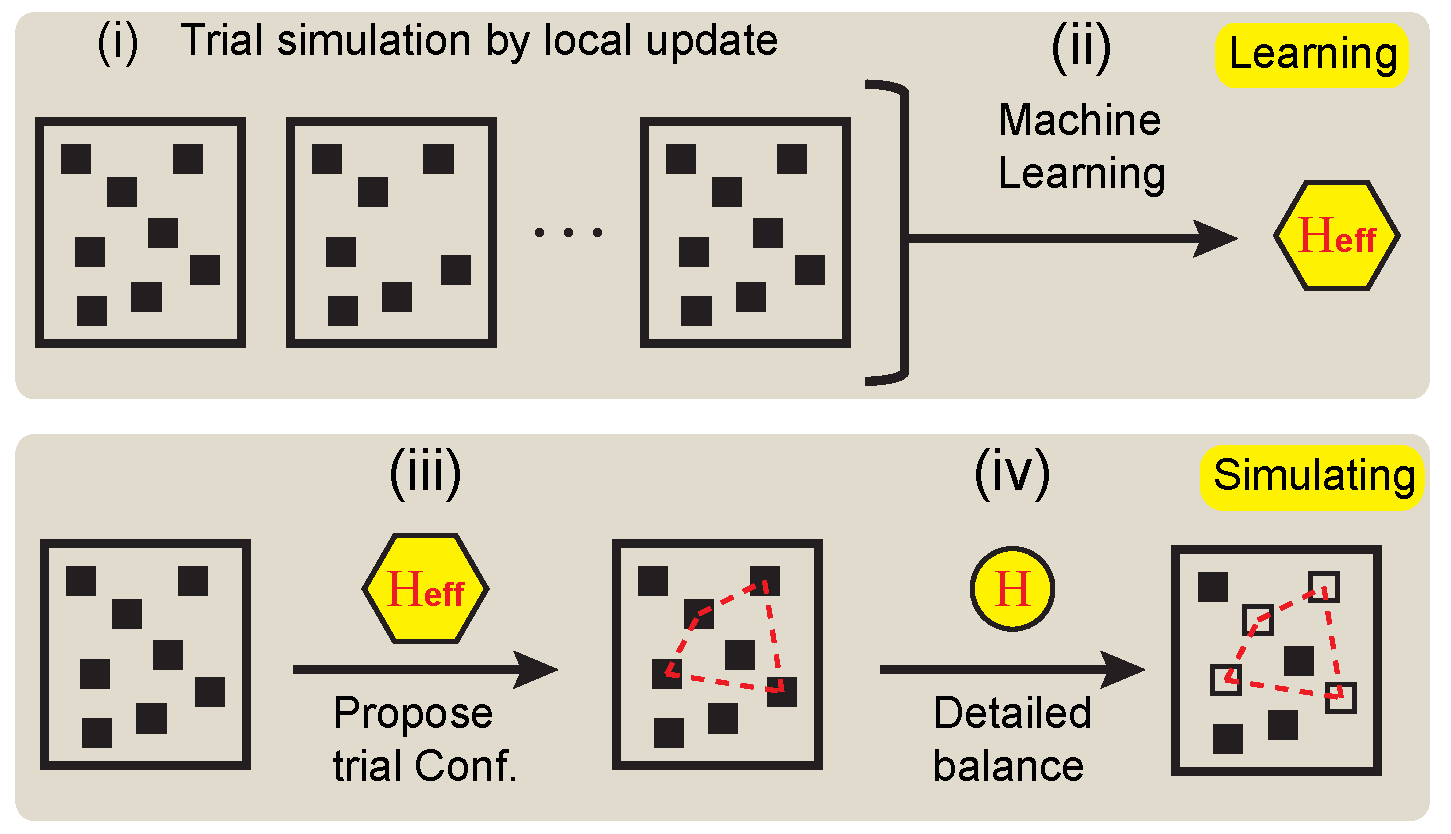
\includegraphics[width=.8\textwidth]{Fig1}
  \end{center}
\end{frame}

\begin{frame}
  \frametitle{Unsupervised machine learning}
  \begin{itemize}
    \item The linear regression we just did can be viewed as an unsupervised machine learning.
    \item Unsupervised ML: learning the underlying distribution from a sample of configurations.
    \item We pretend that we didn't know $H$, and learn a simpler model $H_{\text{eff}}$.
    \item The learned model describes the low-energy effective theory, where the high-energy fluctuations are treated as noise in the sample.
    \item Can incorporate more advanced ML models and algorithms.
  \end{itemize}
\end{frame}


\section{Example: Ising Model and Cluster Update}

\begin{frame}
  \frametitle{Example:}
  \begin{itemize}
    \item The model:
    \[H= - J_1 \sum_{\langle ij\rangle} s_i s_j - J_2 \sum_{ijkl \in \qedsymbol } s_i s_j s_k s_l.\]
    \item The effective model:
    \[H_{\text{eff}} = -J_1^{\text{eff}}\sum_{\langle ij\rangle} s_i s_j.\]
    \item We consider $J_1=1$, $J_2=0.2$.
    \item An Ising transition at $T_c=2.493$.\\
    {\small Ising model without $J_2$ has $T_c=2.269$.}
  \end{itemize}
\end{frame}

\begin{frame}
  \frametitle{Learning the effective model}
    \begin{enumerate}
      \item Generate a sample using the local update.
      \item Perform a linear regression,
      \[  H_{\text{eff}} = J_1^{\text{eff}}\sum_{\langle ij\rangle}S_iS_j+E_0.\]
    \end{enumerate}
    \centering
    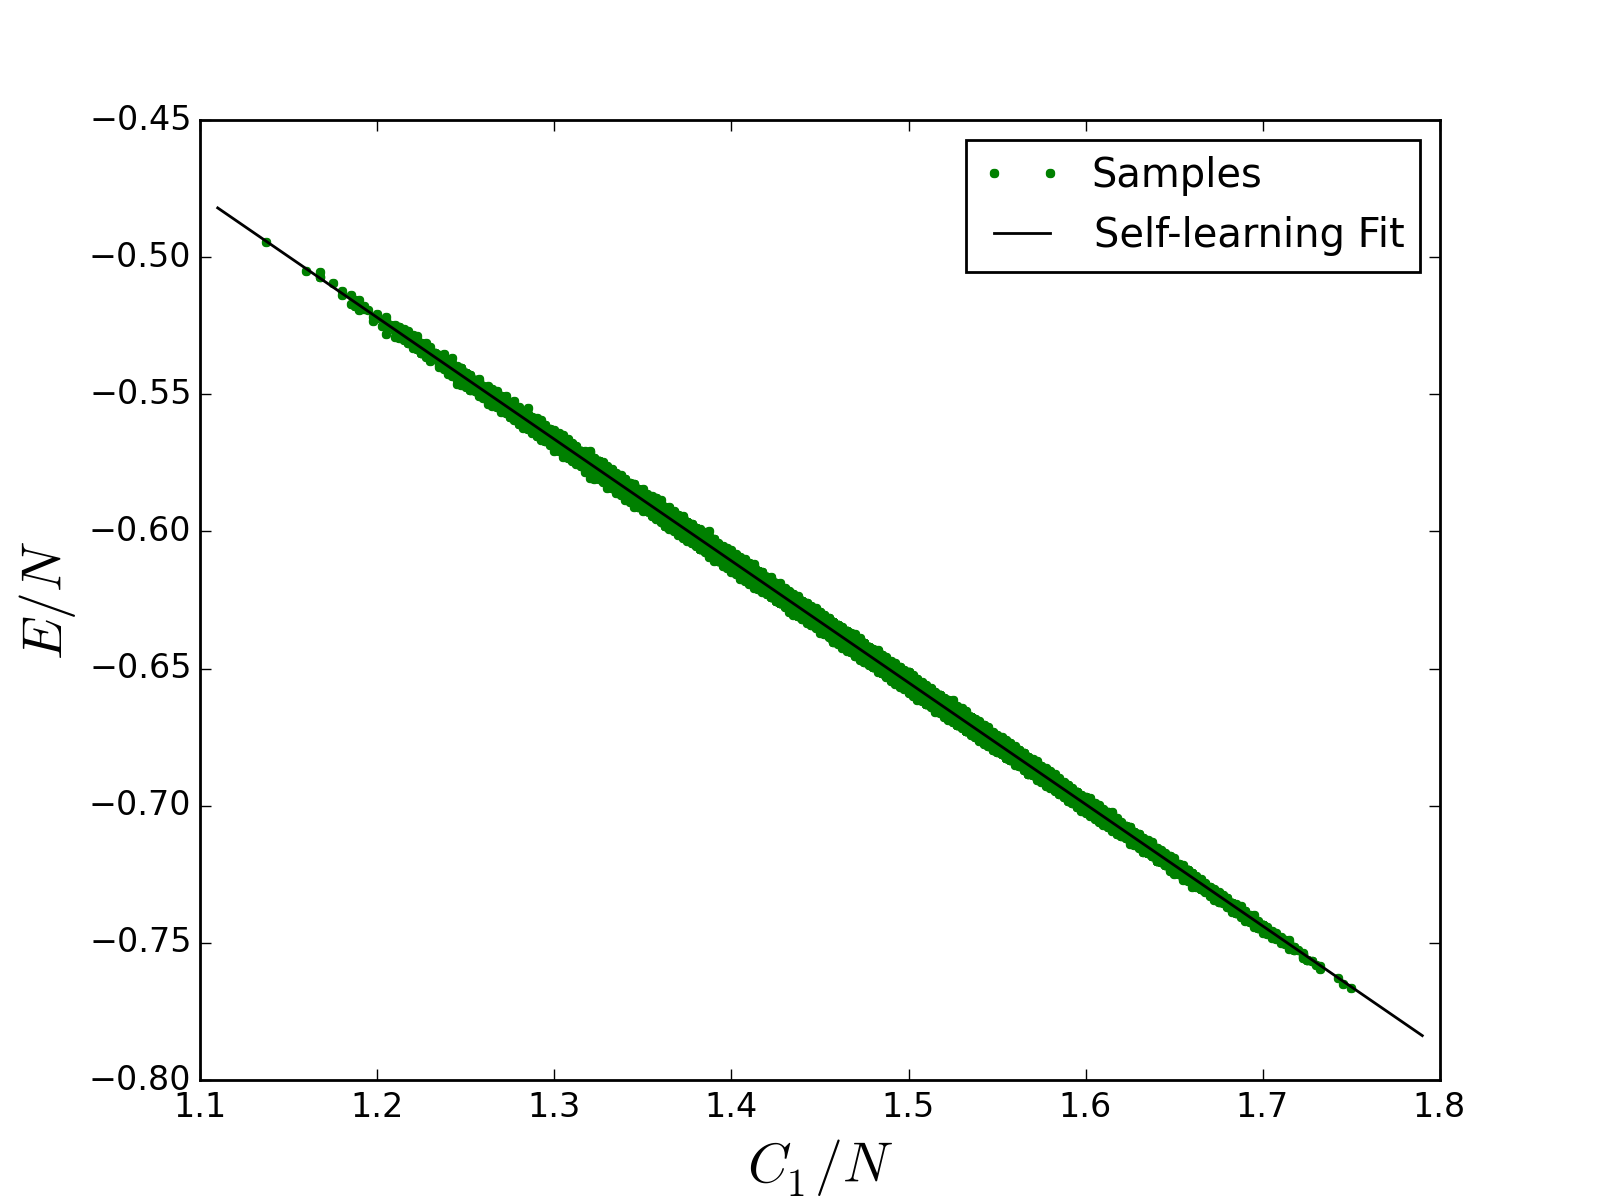
\includegraphics[width=.5\columnwidth]{dist_fit.png}
\end{frame}

%\begin{frame}
%  \frametitle{Learning the effective model}
%    \begin{enumerate}
%      \item Generate a sample using the local update, at $T=5>T_c$.
%      \item Perform a linear regression,
%      \[  H_{\text{eff}} = J_1^{\text{eff}}\sum_{\langle ij\rangle}S_iS_j+E_0.\]
%      \item $J_1^{\text{eff}} = 1.0726$.
%      \item Generate another sample using the self-learning update, at $T=T_c$.
%      \item $J_1^{\text{eff}}=1.1064$.
%    \end{enumerate}
%\end{frame}

\begin{frame}
  \frametitle{Autocorrelation time}
  \centering
  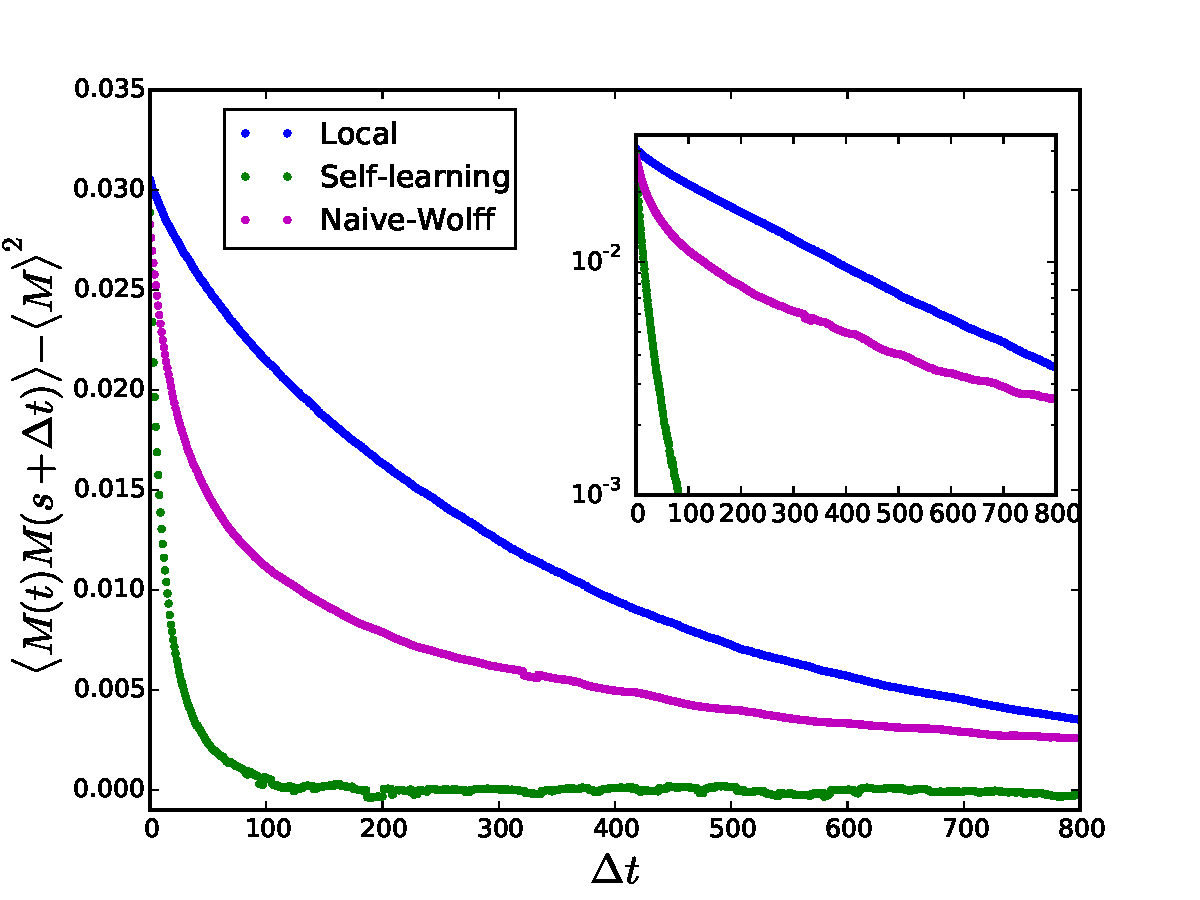
\includegraphics[width=.6\textwidth]{auto_decay}\\
  System size $40\times40$.
\end{frame}

\section{Example: Bosonic Model and Cumulative Update}

\begin{frame}{Determinant Monte Carlo: computational cost}
\begin{itemize}
  \item Fermion coupling to (auxiliary) bosonic field.
  \[H=-\sum_{ij}t_{ij}c_i^\dagger c_j
  +\sum_i\sigma_ic_i^\dagger c_i
  +H[\sigma].\]
  \item Simulation: use bosonic field as configurations.
  \[\mathcal C=\{\sigma_i(t)\}, i=1,\ldots N;0<t<\beta.\]
  \item Weight of each configuration $W(\mathcal C)$: integrate out the fermions.
  \item Computational cost: $\beta N^3$:\\
  \emph{\small Computing the determinant of the product of $\beta$ $N\times N$ matrices.}
  \item Fast update: $\beta N^3$ for $\beta N$ steps of local updates.
  \item Generating two independent configurations: $\beta N^3\tau_L$.
  \item Critical slow-down:\\ when $\sigma_i$ goes through a critical point, $\tau_L\gg1$, very slow.
\end{itemize}
\end{frame}

\begin{frame}{Cumulative update}
  \begin{itemize}
    \item Idea: replace $W(\mathcal C)$ by $W_{\text{eff}}(\mathcal C)$, which is much faster to evaluate.
    \item Local updates guided by $W_{\text{eff}}(\mathcal C)$:
    \[\mathcal C\Rightarrow\mathcal D:
    \mathcal C\rightarrow\mathcal C_1\cdots\rightarrow\mathcal C_{i-1}\rightarrow\mathcal C_i\rightarrow\mathcal C_{i+1}\rightarrow\cdots\rightarrow\mathcal C_M\rightarrow\mathcal D.\]
    \[\frac{p(\mathcal C_i\rightarrow\mathcal C_{i+1})}{p(\mathcal C_{i+1}\rightarrow\mathcal C_i)}=\frac{W_{\text{eff}}(\mathcal C_{i+1})}{W_{\text{eff}}(\mathcal C_i)}\]
    %\item For each path:
    %\[\frac{p(\mathcal C\rightarrow\mathcal C_1)\cdots
    %p(\mathcal C_i\rightarrow\mathcal C_{i+1})
    %p(\mathcal C_M\rightarrow\mathcal D)}
    %{p(\mathcal C_1\rightarrow\mathcal C)\cdots
    %p(\mathcal C_{i+1}\rightarrow\mathcal C_i)
    %p(\mathcal D\rightarrow\mathcal C_M)}
    %=\frac{W^\prime(\mathcal C_1)}{W^\prime(\mathcal C)}
    %\frac{W^\prime(\mathcal C_2)}{W^\prime(\mathcal C_1)}
    %\cdots\frac{W^\prime(\mathcal C_M)}{W^\prime(\mathcal C_{M-1})}
    %\frac{W^\prime(\mathcal D)}{W^\prime(\mathcal C_M)}
    %=\frac{W^\prime(\mathcal D)}{W^\prime(\mathcal C)}.\]
    \item Selection rate and acceptance ratio:
    \[\frac{q(\mathcal C\rightarrow D)}
    {q(\mathcal D\rightarrow\mathcal C)}
    %=\frac{p(\mathcal C\Rightarrow D)}
    %{p(\mathcal D\Rightarrow\mathcal C)}
    %=\frac{\sum_{\mathcal C_i}p(\mathcal C\rightarrow\mathcal C_1)\cdots
    %p(\mathcal C_i\rightarrow\mathcal C_{i+1})
    %p(\mathcal C_M\rightarrow\mathcal D)}
    %{\sum_{\mathcal C_i}p(\mathcal C_1\rightarrow\mathcal C)\cdots
    %p(\mathcal C_{i+1}\rightarrow\mathcal C_i)
    %p(\mathcal D\rightarrow\mathcal C_M)}
    =\frac{W_{\text{eff}}(\mathcal D)}{W_{\text{eff}}(\mathcal C)},\quad
    \alpha(\mathcal C\rightarrow \mathcal D)=\min\left\{1, \frac{W(\mathcal D)}{W(\mathcal C)}
    \frac{W_{\text{eff}}(\mathcal C)}{W_{\text{eff}}(\mathcal D)}\right\}\simeq1.\]
		\item Choose good $W^\prime$ and $M\geq\tau_L$: $\tau_{CU}\sim1$.
    \item Computational cost: $\beta N^3\tau\rightarrow \beta N^3$.
  \end{itemize}
\end{frame}

\begin{frame}{Constructing effective weights}
\begin{enumerate}
  \item Physical intuition: bosonic effective model of $W_{\text{eff}}[\sigma]$
  + Linear Regression.\\
  \emph{Works best for gapped fermions.}
  \[H=-\sum_{ij}t_{ij}c_{i\alpha}^\dagger c_{j\alpha}
  +\sum_i\sigma_ic_{i\alpha}^\dagger\sigma^z_{\alpha\beta} c_{i\beta}
  +H[\sigma]\]
  \[W_{\text{eff}}[\sigma]=\sum_{ij}J_{ij}\sigma_i\sigma_j.\]
  \item Machine Learning models: Restricted Boltzmann Machine, Neural Networks, etc.
\end{enumerate}
\end{frame}

\section{SLMC in action: using SLMC to solve real-world problems}

\begin{frame}{SLMC in action: large scale DQMC}
\begin{itemize}
  \item Zi-Hong Liu, Xiao-Yan Xu, Yang Qi, Kai Sun and Zi-Yang Meng, arXiv:1706.10004.
  \item Fermion + boson model, new critical universality. Simulated at the critical point.
  \item SLMC: $L=24\rightarrow30$.
\end{itemize}
\begin{center}
  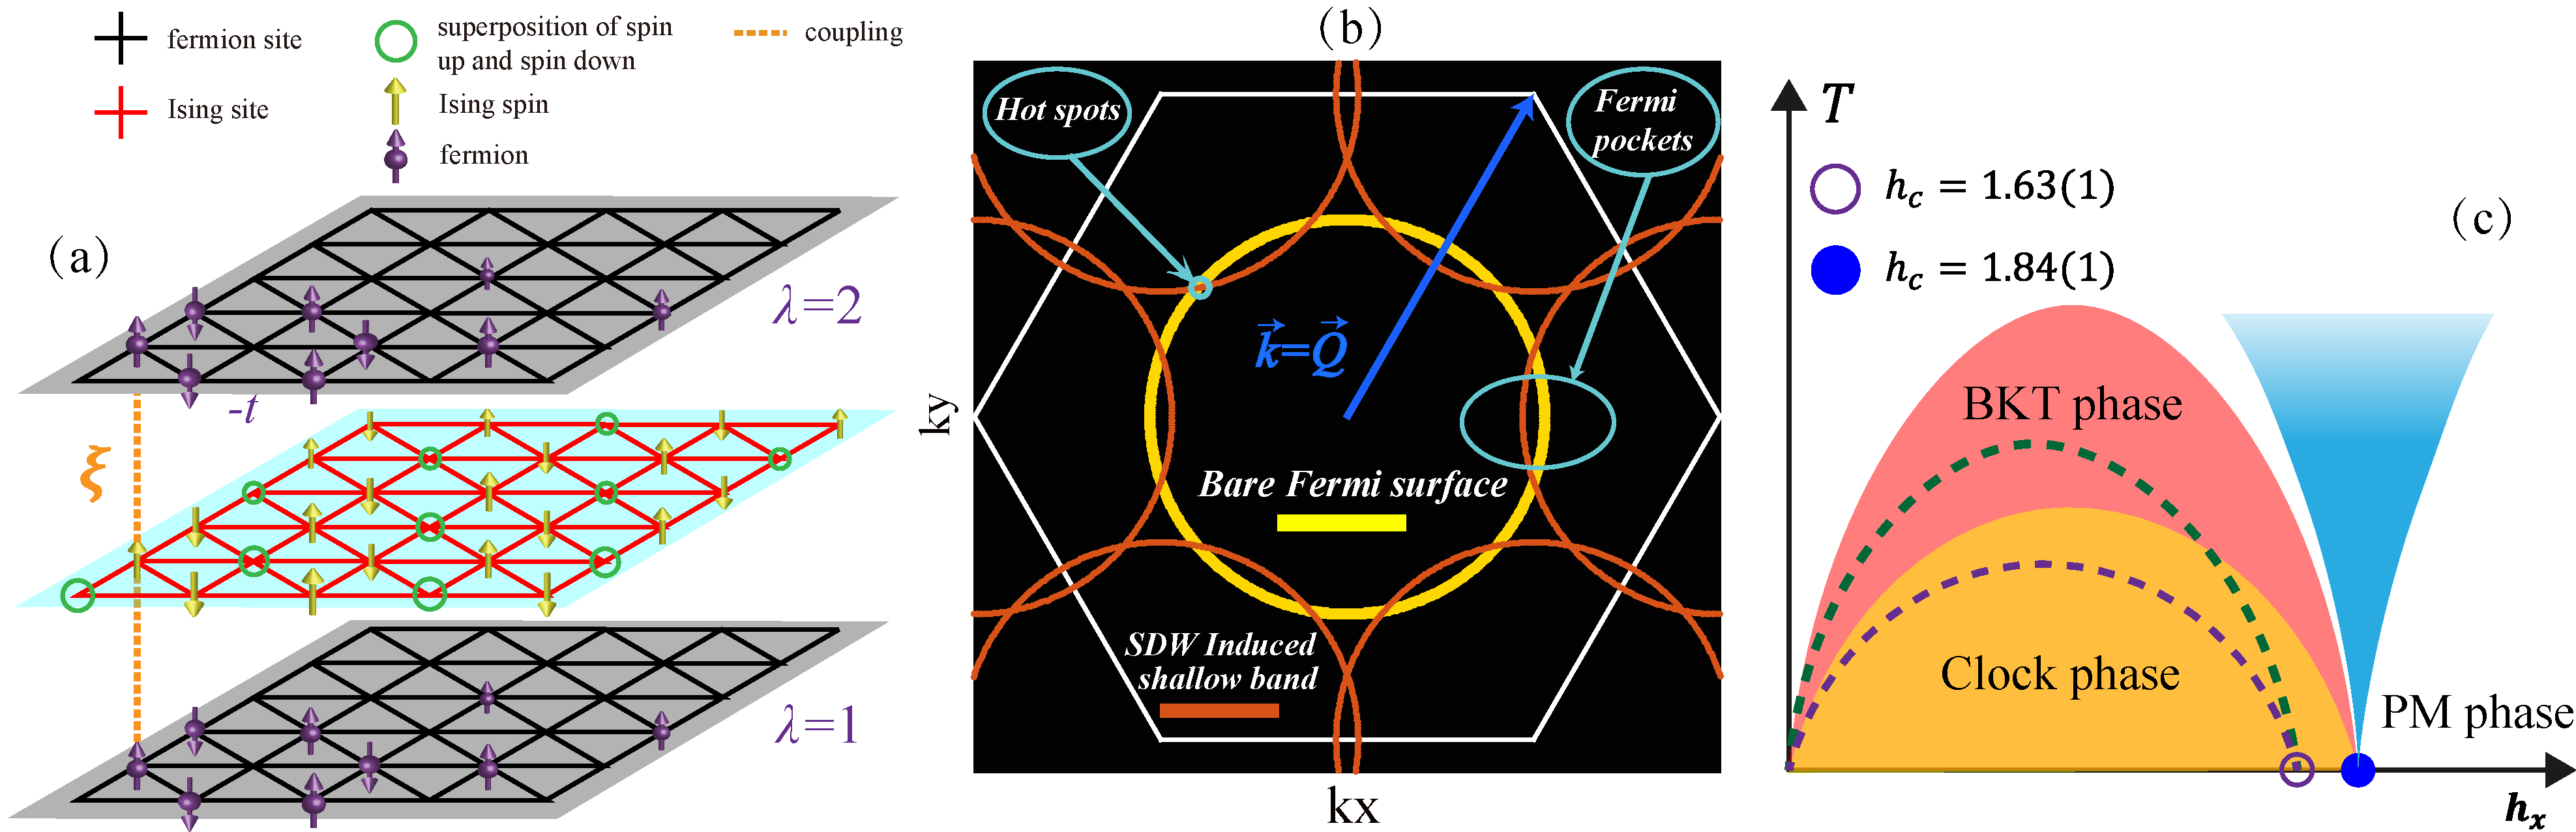
\includegraphics[width=.6\textwidth]{combine}
  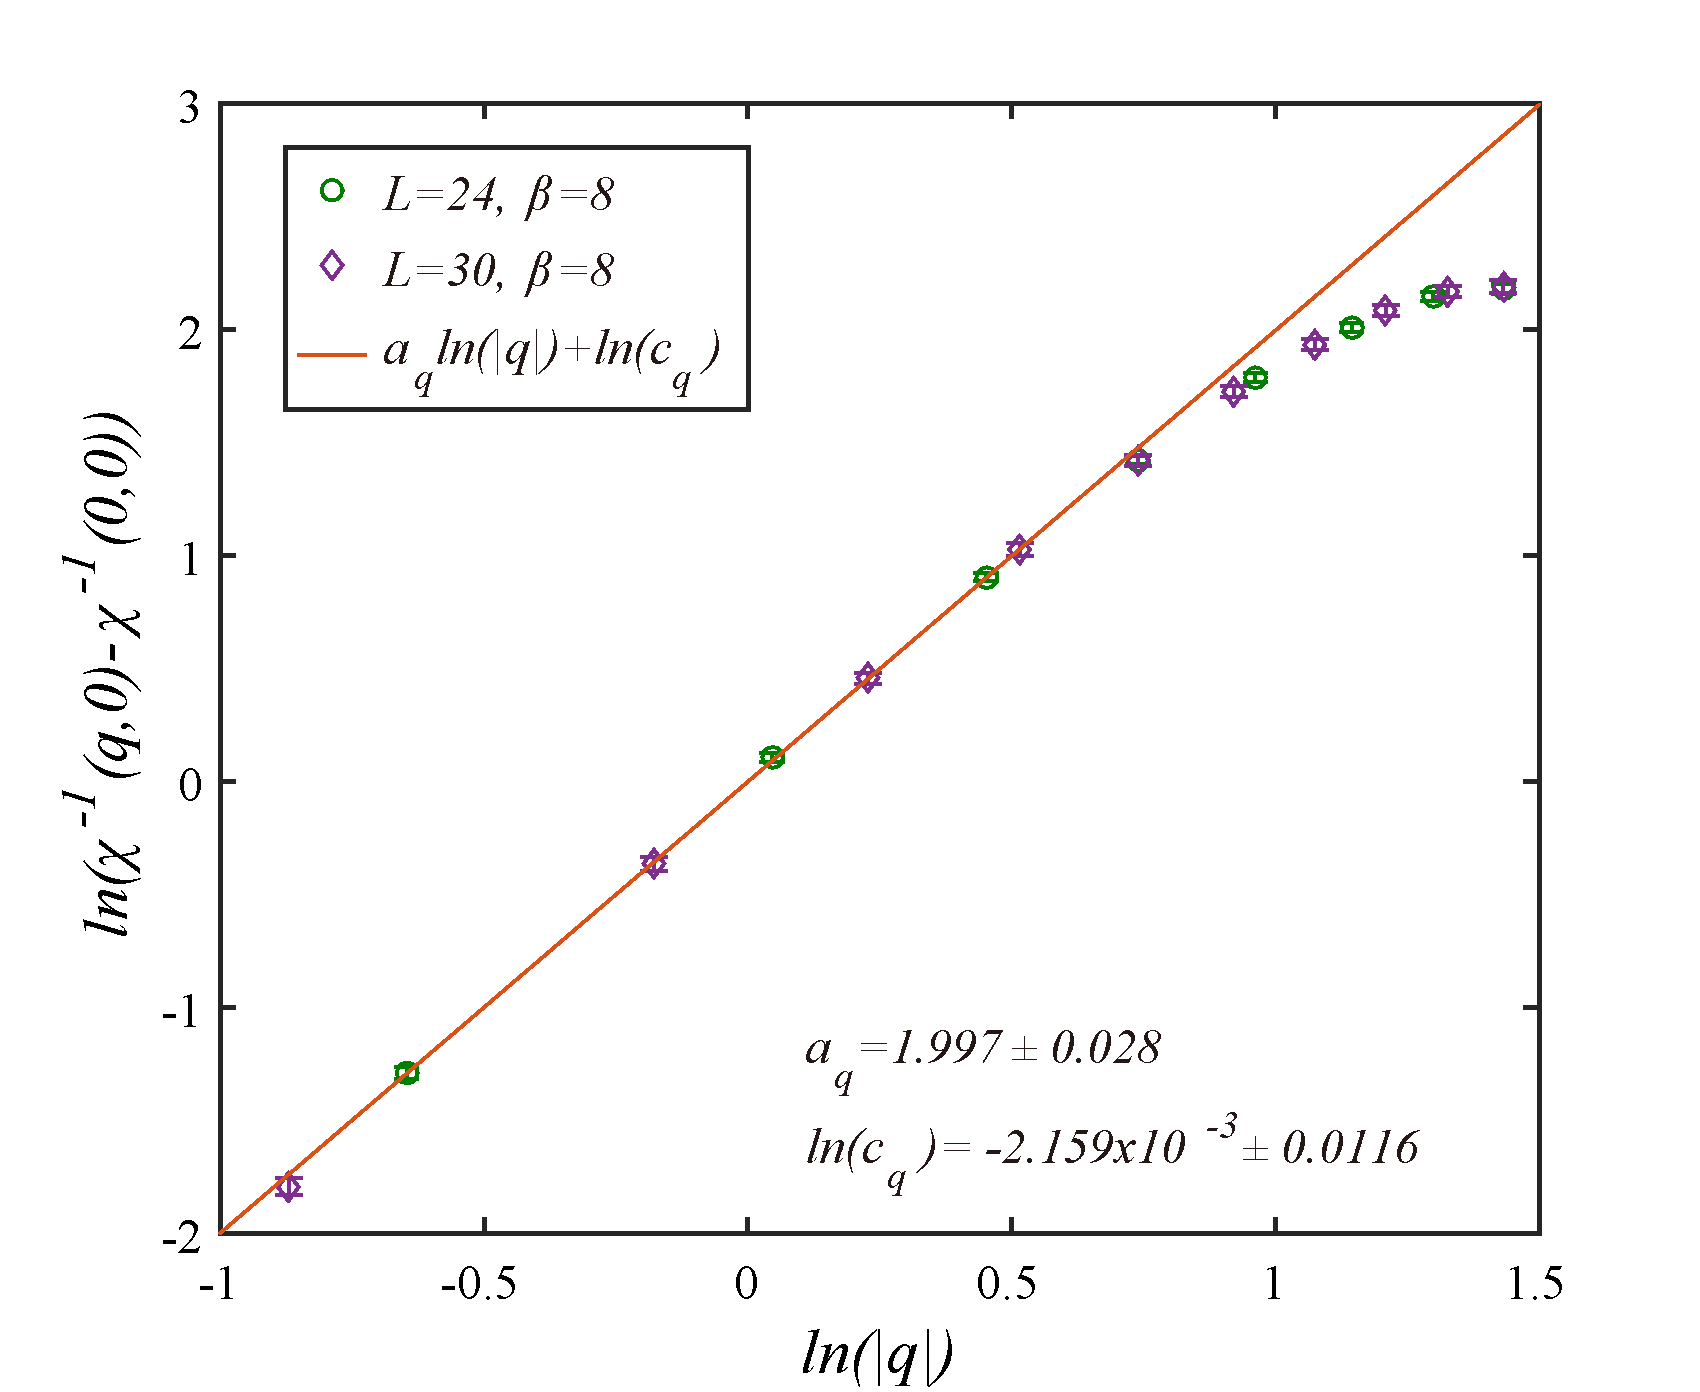
\includegraphics[width=.4\textwidth]{chi-q-fit}
\end{center}
\end{frame}

\begin{frame}{SLMC in action: EQMC}
\begin{itemize}
	\item Zi Hong Liu, Xiao Yan Xu, Yang Qi, Kai Sun and Zi Yang Meng, arXiv:1801.00127.
	\item EMUS-QMC: Elective Momentum Ultra-Size Quantum Monte Carlo Method.
	\item To study a quantum critical point: only keep fermion modes near the ``hot spots''.
	\item Model becomes \emph{nonlocal}: cannot perform local updates.
	\item SLMC provides a generic way to construct global updates.
\end{itemize}
\begin{center}
	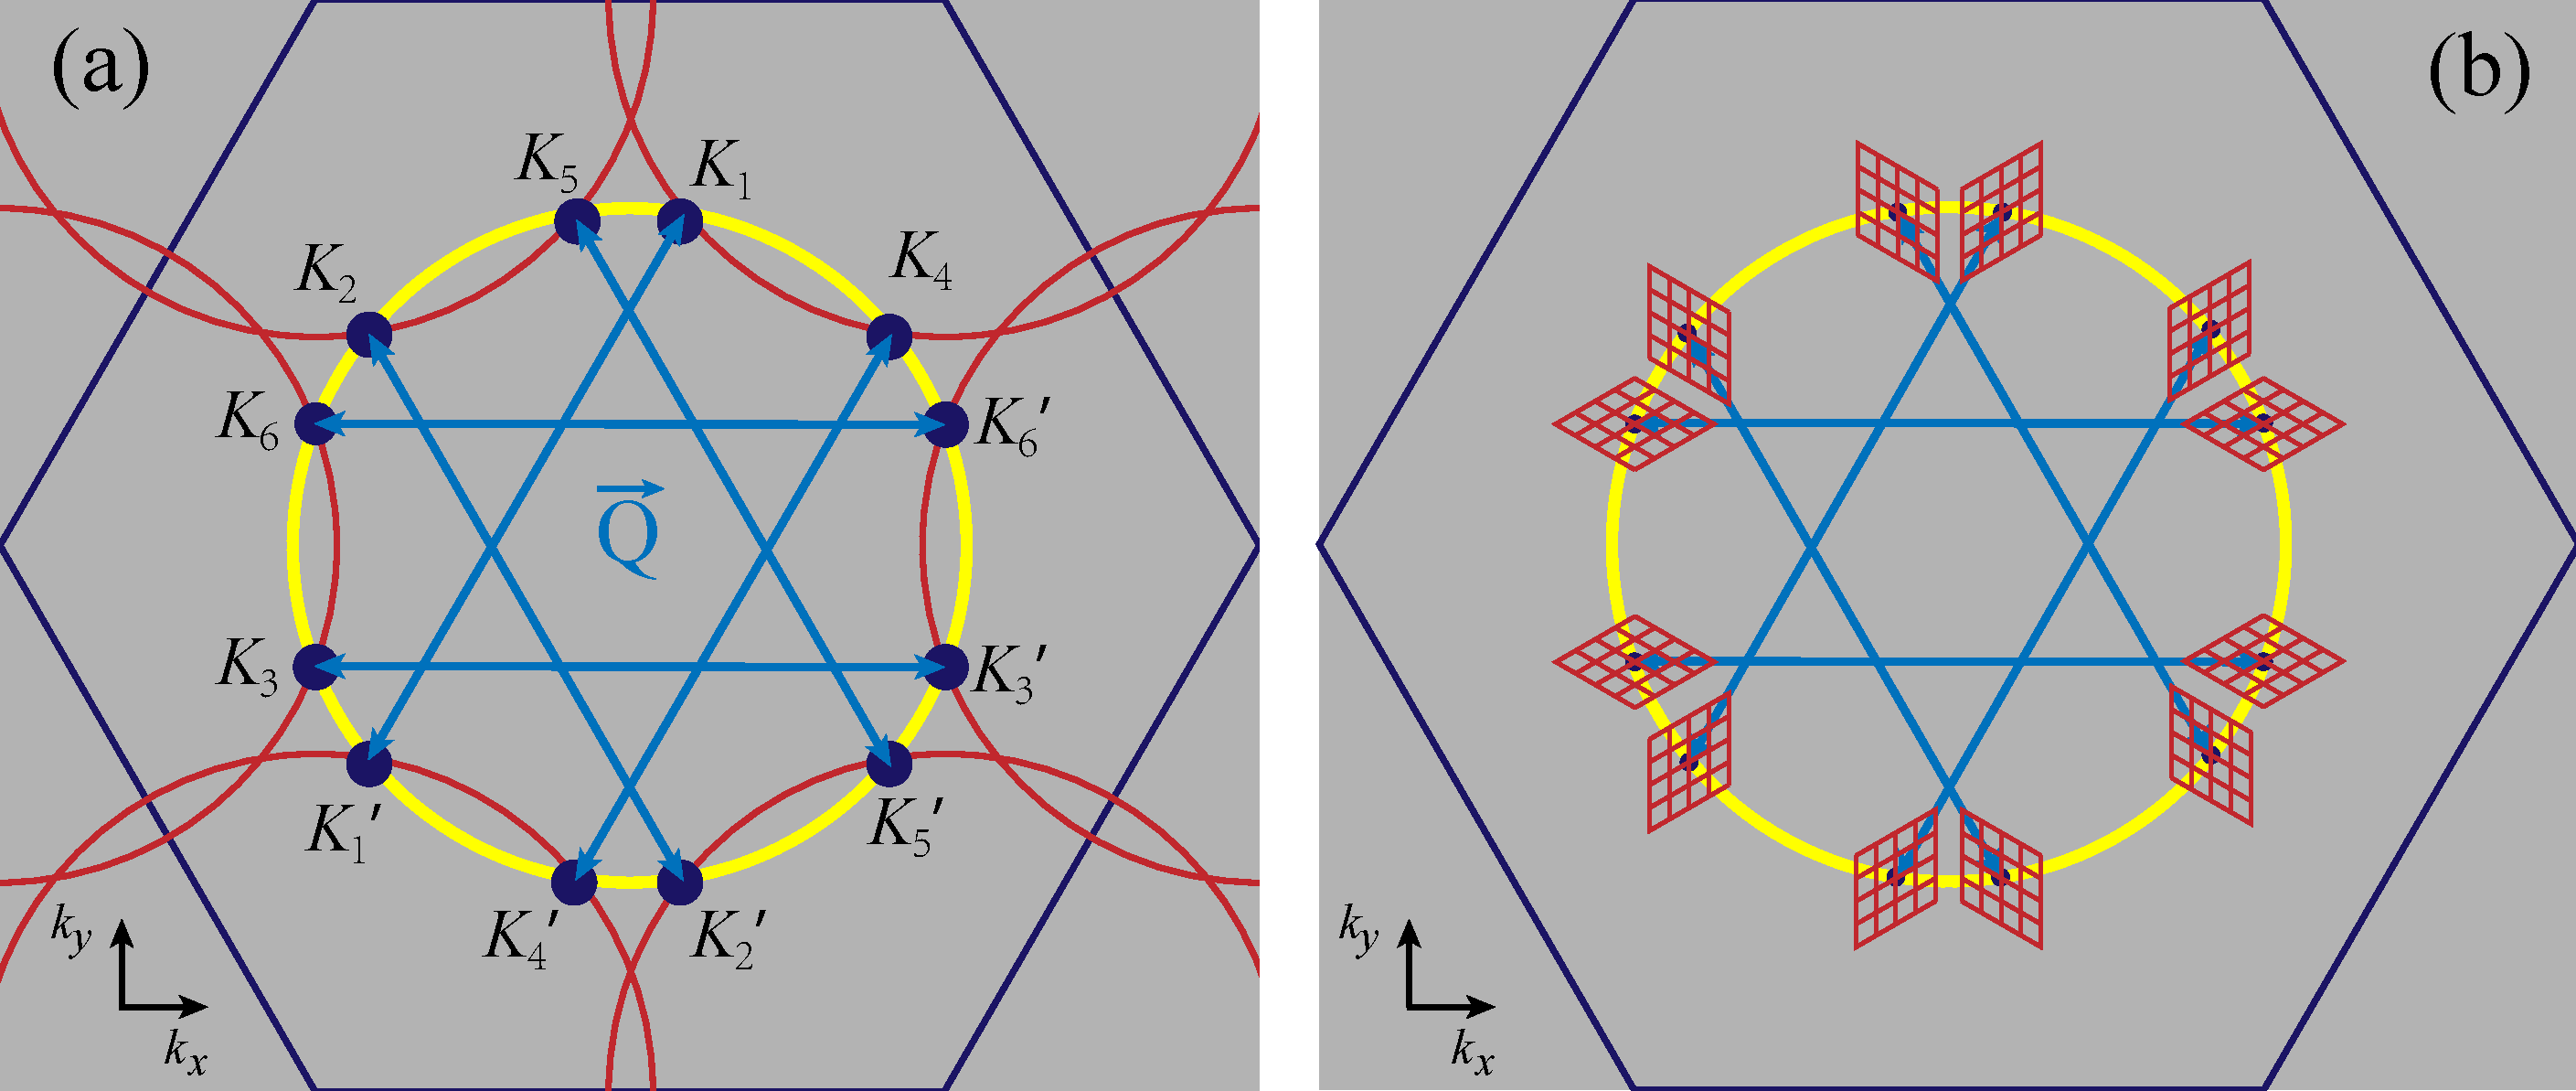
\includegraphics[width=.8\textwidth]{../eqmc/kmeshtri}
\end{center}
\end{frame}

\begin{frame}{SLMC in action: the Holstein Model}
	\begin{itemize}
		\item Chuang Chen, Xiao Yan Xu, Junwei Liu, George Batrouni, Richard Scalettar and Zi Yang Meng, arXiv:1802.06177.
		\item Electron-Phonon coupling:
		\[H=H_{\text{el}}+H_{\text{ph}}+H_{\text{el-ph}}
		=-t\sum_{\langle ij\rangle\sigma}c_{i\sigma}^\dagger c_{j\sigma}
		+\sum_i\left(\frac12M\Omega^2X_i^2+\frac1{2M}P_i^2\right)
		+g\sum_{i\sigma}c_{i\sigma}^\dagger c_{i\sigma}X_i.\]
		\item Effective model: $W_{\text{eff}}$ is a bosonic function of $X_{i\tau}$, constructed using symmetries of the model to reduce the \# of fitting parameters.
	\end{itemize}
	\begin{center}
		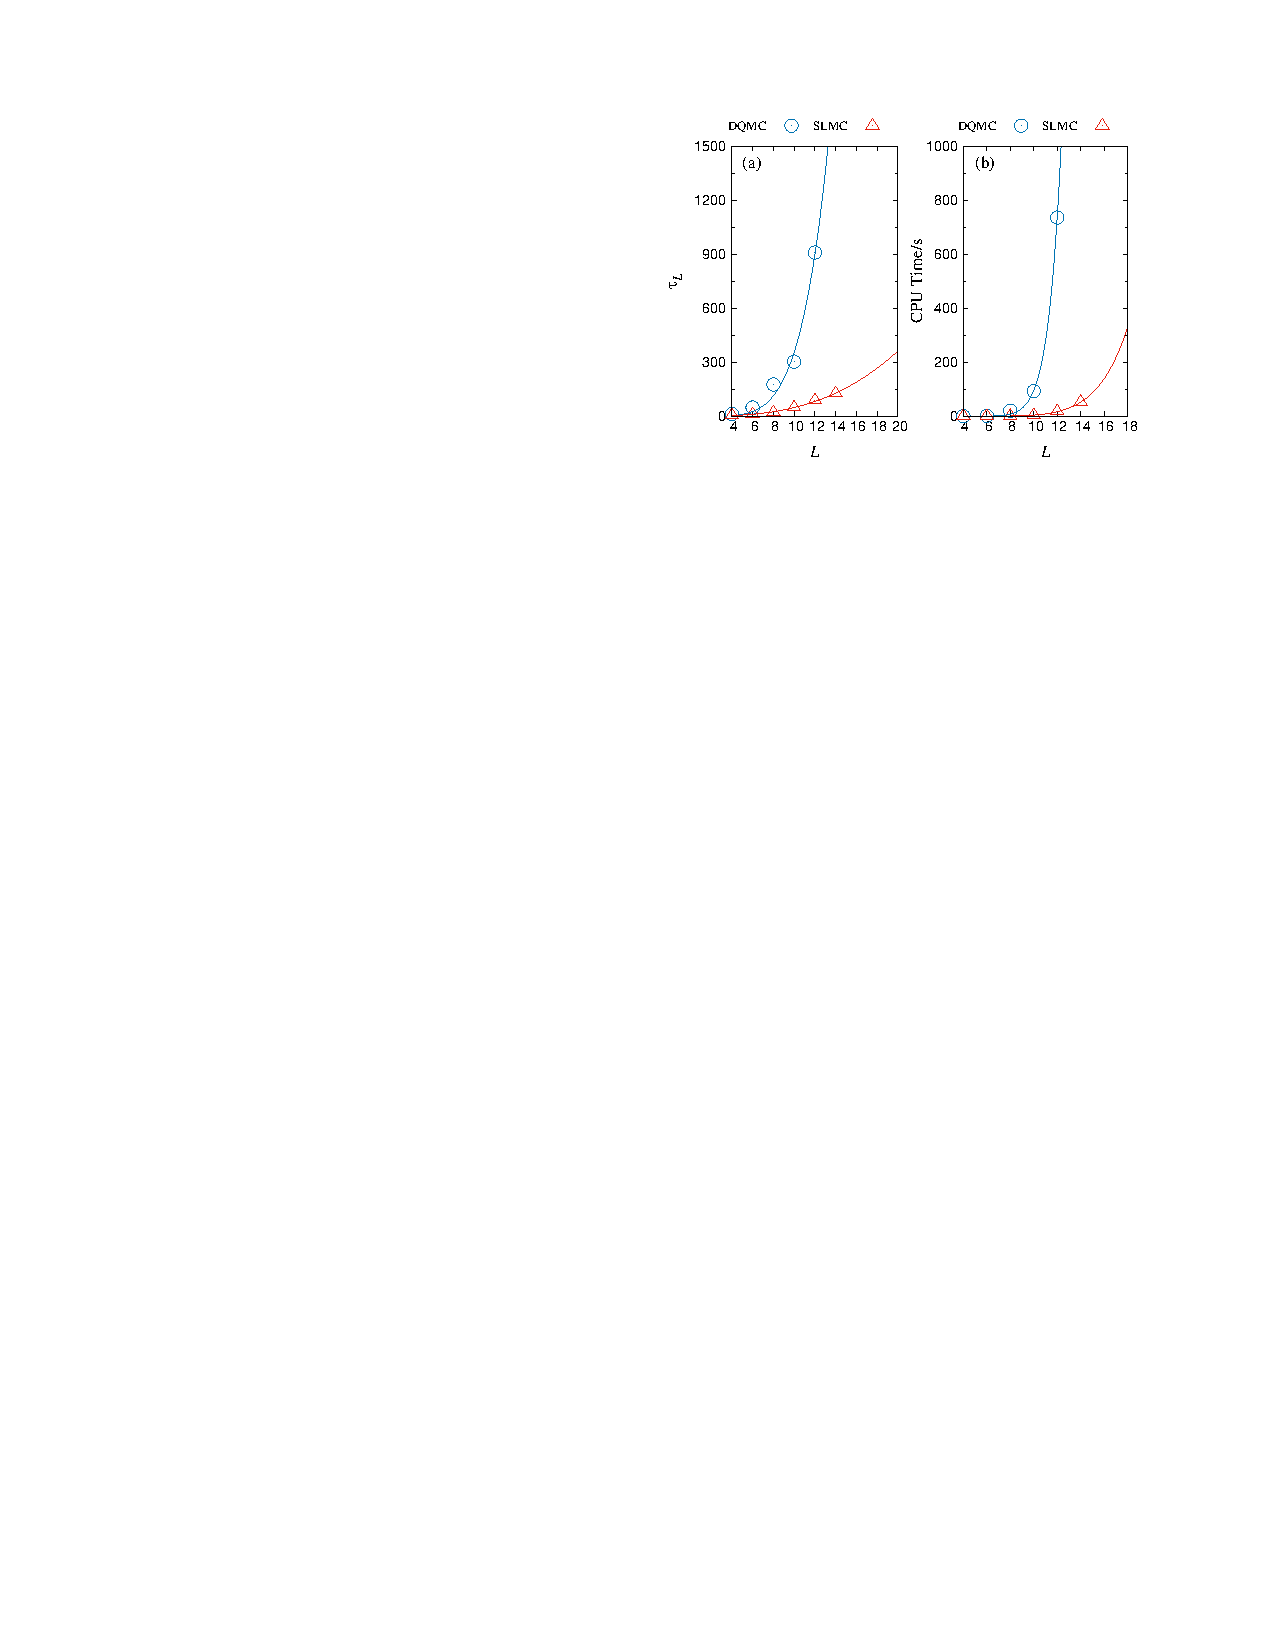
\includegraphics[width=.35\textwidth]{holstein}
	\end{center}
\end{frame}

\begin{frame}{SLMC with Deep Neural Networks}
\begin{itemize}
	\item Huitao Shen, Junwei Liu and Liang Fu, arXiv:1801.01127.
	\item 1D single-impurity Andensen Model.
	\item $W_{\text{eff}}$: given by a Deep Neural Network.
\end{itemize}
\begin{center}
	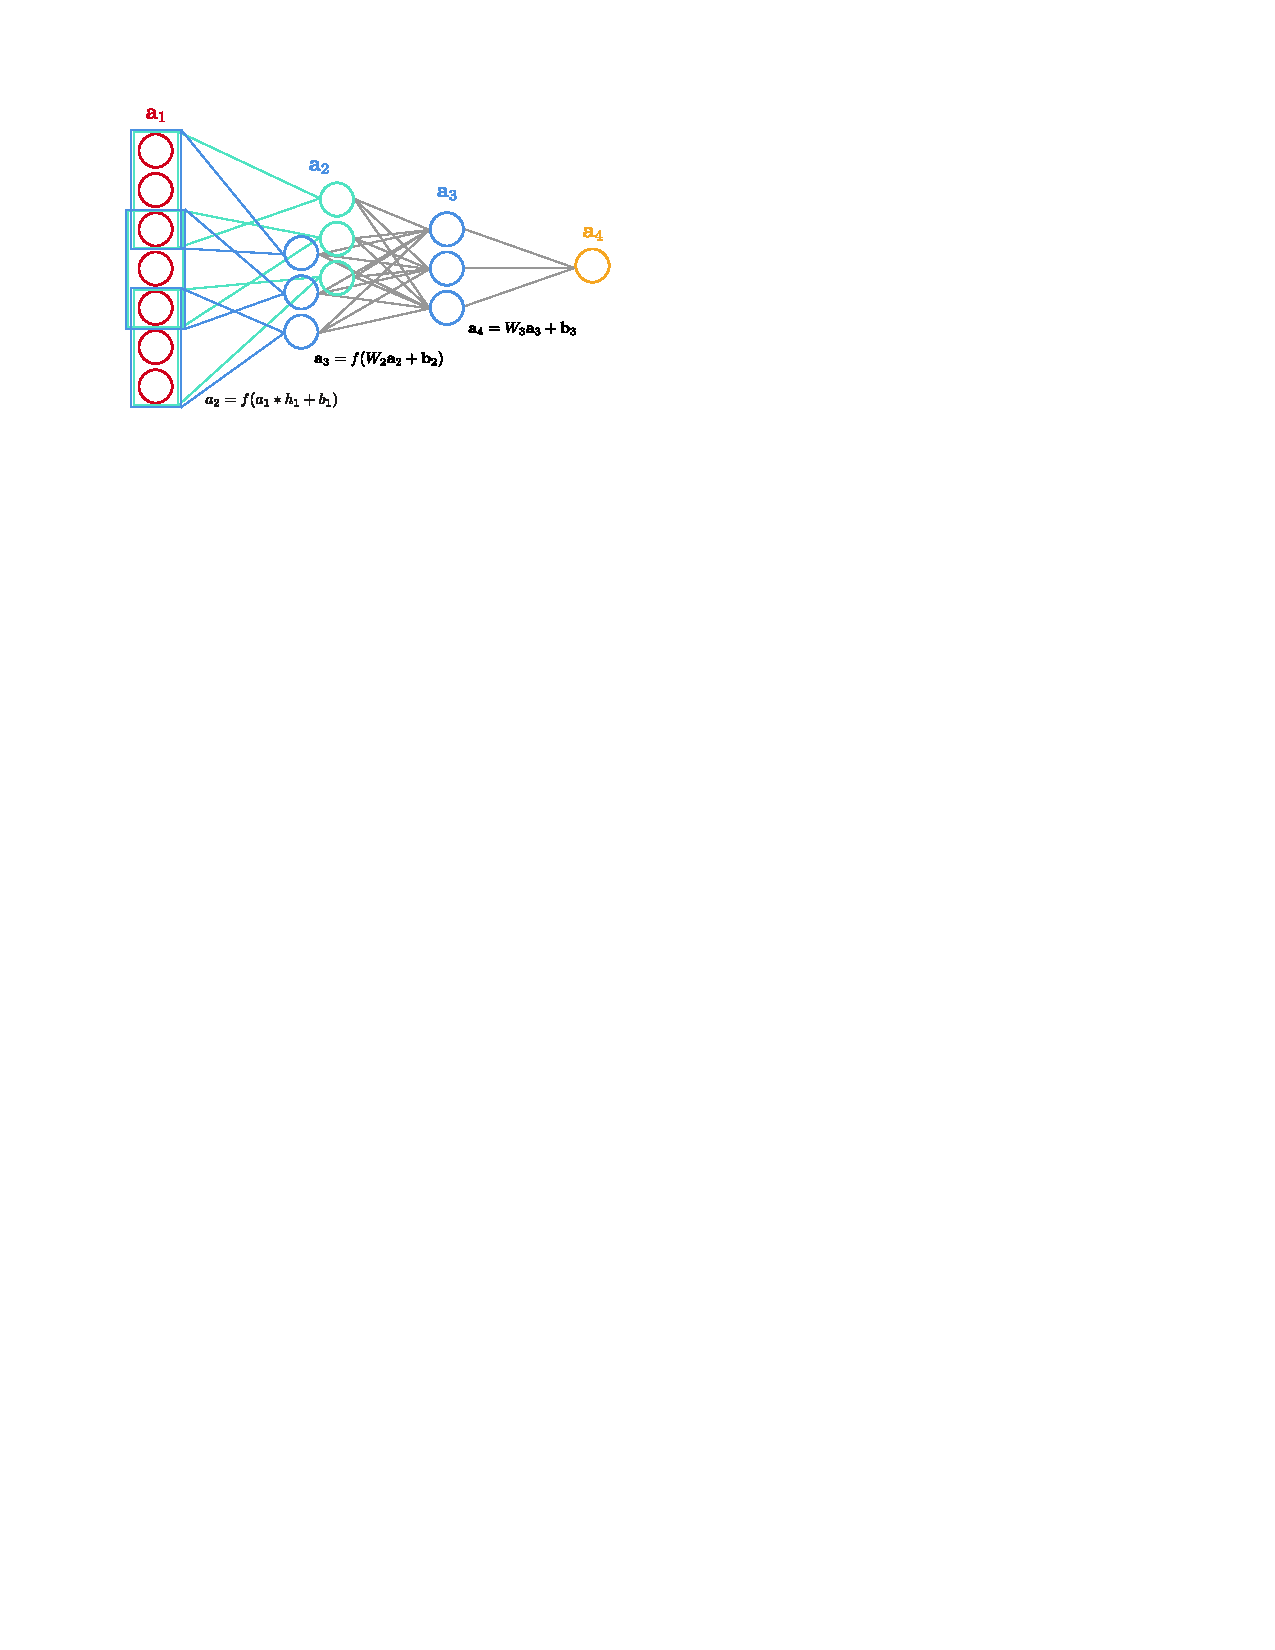
\includegraphics[width=.6\textwidth]{dnn}
\end{center}
\end{frame}

\begin{frame}{Conclusion}
	\begin{itemize}
		\item Self-Learning Monte Carlo:
		\begin{enumerate}
			\item Train an effective model using a trail run.
			\item Use the effective model to select a new configuration.
			\item Use the original model to accept/reject.
		\end{enumerate}
		\item The accuracy of the effective model does not affect the accuracy of the result.
		\item Cumulative update: for DQMC (fermion problems), use a bosonic effective model + many local updates.
		\item Useful when local-update is slow and global-update is hard to construct by hand.
		\item Future directions:
		\begin{enumerate}
			\item Application to real-world models.
			\item Use more advanced models from ML.
		\end{enumerate}
	\end{itemize}
\end{frame}

\end{document}
